\documentclass[dvipsnames,colorlinks]{beamer}

\usepackage[utf8]{inputenc}
\usepackage{fancybox}
\usepackage{environ,fancyvrb,xspace,empheq}

\usepackage{tikz}
\usetikzlibrary{arrows.meta,decorations.markings,decorations.pathreplacing,fadings,positioning}

\newcommand{\ds}{\displaystyle}
\newcommand{\grad}{\nabla}
\newcommand{\ih}{\boldsymbol{\hat{\textbf{\i}}}}
\newcommand{\jh}{\boldsymbol{\hat{\textbf{\j}}}}
\newcommand{\vF}{\boldsymbol{\vec{\textbf{F}}}}

\newcommand{\Matlab}{\textsc{Matlab}\xspace}

\newcommand\enumnum[1]{{\renewcommand{\insertenumlabel}{#1}%
      \usebeamertemplate{enumerate item} \,}}

\newcommand{\bA}{\mathbf{A}}
\newcommand{\bF}{\mathbf{F}}
\newcommand{\bX}{\mathbf{X}}


\beamertemplatenavigationsymbolsempty

\title{8.1 Linear systems of first-order ODEs: \\ basics and forms}

\subtitle{a lecture for MATH F302 Differential Equations}

\author{Ed Bueler, Dept.~of Mathematics and Statistics, UAF}

\date{Fall 2023}


\usetheme{Pittsburgh}


\begin{document}

\setbeamertemplate{itemize item}{$\bullet$}
\setbeamertemplate{itemize subitem}{$\circ$}


\begin{frame}
\titlepage

\centerline{\tiny for textbook: \, D. Zill, \emph{A First Course in Differential Equations with Modeling Applications}, 11th ed.}
\end{frame}


\begin{frame}{first-order systems}

\begin{itemize}
\item we have already seen the most general form of a system of ODEs (\S3.3):
\begin{align*}
\frac{dx_1}{dt} &= g_1(t,x_1,x_2,\dots,x_n) \\
\frac{dx_2}{dt} &= g_2(t,x_1,x_2,\dots,x_n) \\
                &\qquad \vdots \\
\frac{dx_n}{dt} &= g_n(t,x_1,x_2,\dots,x_n)
\end{align*}
     \begin{itemize}
     \item my claim in \S3.3: everything is modeled this way
     \end{itemize}
\item Chapter 8 is about a special case:

\centerline{\alert{suppose variables $x_i$ only appear with first powers}}
\end{itemize}
\end{frame}


\begin{frame}{first-order \emph{linear} systems}

\begin{itemize}
\item a \alert{first-order system of linear ODEs} is
\begin{align*}
\frac{dx_1}{dt} &= a_{11}(t) x_1 + a_{12}(t) x_2 + \dots + a_{1n}(t) x_n + f_1(t) \\
\frac{dx_2}{dt} &= a_{21}(t) x_1 + a_{22}(t) x_2 + \dots + a_{2n}(t) x_n + f_2(t) \\
                &\qquad \vdots \\
\frac{dx_n}{dt} &= a_{n1}(t) x_1 + a_{n2}(t) x_2 + \dots + a_{nn}(t) x_n + f_n(t)
\end{align*}
     \begin{itemize}
     \item the book calls this the \emph{normal form} of the system

\smallskip
     \item $a_{ij}(t)$ functions are the \emph{coefficients}
         \begin{itemize}
         \item if $a_{ij}(t)$ are independent of time then we say it is a \emph{constant-coefficient} system
         \end{itemize}
     \item $f_i(t)$ are the \emph{source functions}
         \begin{itemize}
         \item if all $f_i=0$ then the system is \emph{homogeneous}
         \end{itemize}
     \end{itemize}
\end{itemize}
\end{frame}


\begin{frame}{examples}

\small
\begin{itemize}
\item consider three example systems from the \href{https://bueler.github.io/math302/assets/slides/3-3.pdf}{\S3.3 slides} and \href{https://drive.explaineverything.com/thecode/XAAUNGS}{video}
\end{itemize}

\noindent \emph{instructions:} identify the coefficients $a_{ij}(t)$ and source functions $f_i(t)$

\begin{itemize}
\item \emph{example 1.}
\begin{align*}
\frac{dx}{dt} &= - 2 x \hspace{70mm} \\
\frac{dy}{dt} &= x - y
\end{align*}
\item \emph{example 2.}
\begin{align*}
\frac{dx_1}{dt} &= -0.04 x_1 + 0.02 x_2 \hspace{60mm} \\
\frac{dx_2}{dt} &= 0.04 x_1 - 0.07 x_2 + 0.03 x_3 \\
\frac{dx_3}{dt} &= 0.05 x_2 - 0.05 x_3
\end{align*}
\end{itemize}
\end{frame}


\begin{frame}{examples, cont.}

\small
\begin{itemize}
\item \emph{example 3.}
\begin{align*}
y' &= u \hspace{75mm} \\
u' &= v \\
v' &= w \\
w' &= 4w-7v-10u+y+\sin(3t)
\end{align*}
\end{itemize}

\vspace{40mm}
\end{frame}


\begin{frame}{matrix form}

\begin{itemize}
\item a first-order linear system
\small
\begin{align*}
\frac{dx_1}{dt} &= a_{11}(t) x_1 + a_{12}(t) x_2 + \dots + a_{1n}(t) x_n + f_1(t) \\
                &\qquad \vdots \\
\frac{dx_n}{dt} &= a_{n1}(t) x_1 + a_{n2}(t) x_2 + \dots + a_{nn}(t) x_n + f_n(t)
\end{align*}
\normalsize
\item is usually written
    $$\frac{d}{dt} \begin{pmatrix} x_1 \\ x_2 \\ \vdots \\ x_n \end{pmatrix} = \begin{pmatrix}
a_{11} & a_{12} & \dots & a_{1n} \\
a_{21} & a_{22} &       & a_{2n} \\
 \vdots&        & \ddots& \vdots \\
a_{n1} & a_{n2} & \dots & a_{nn}
\end{pmatrix}     \begin{pmatrix} x_1 \\ x_2 \\ \vdots \\ x_n \end{pmatrix} +  \begin{pmatrix} f_1 \\ f_2 \\ \vdots \\ f_n \end{pmatrix}$$
\item or
    $$\bX' = \bA \bX + \bF$$
\end{itemize}
\end{frame}


\begin{frame}{a matrix times a vector}

\begin{itemize}
\item so: \alert{recall matrix-vector multiplication!}
\item \emph{example 4.}  compute the product
    $$\begin{pmatrix} 2 & -3 & -2 \\ 1 & 0 & 5 \\ 4 & 1 & -1\end{pmatrix} \begin{pmatrix} 1 \\ 1 \\ 2 \end{pmatrix} = \hspace{70mm}$$

\vspace{15mm}
\item \emph{example 5.}  compute
    $$\begin{pmatrix} 3 & -2 \\ 1 & 4 \end{pmatrix} \begin{pmatrix} -1 \\ 0 \end{pmatrix} +  \begin{pmatrix} 4 \\ 2 \end{pmatrix} = \hspace{70mm}$$
\end{itemize}

\vspace{15mm}
\end{frame}


\begin{frame}{example matrix forms}

\small
\noindent \emph{instructions:} write the linear systems in matrix form $\bX' = \bA\bX + \bF$

(what is $\bX$? $\bA$? $\bF?$)
\begin{itemize}
\item \emph{example 6.}
\begin{align*}
\frac{dx}{dt} &= - 2 x \hspace{70mm} \\
\frac{dy}{dt} &= x - y
\end{align*}
\item \emph{example 7.}
\begin{align*}
\frac{dx_1}{dt} &= -0.04 x_1 + 0.02 x_2 \hspace{60mm} \\
\frac{dx_2}{dt} &= 0.04 x_1 - 0.07 x_2 + 0.03 x_3 \\
\frac{dx_3}{dt} &= 0.05 x_2 - 0.05 x_3
\end{align*}
\end{itemize}
\end{frame}


\begin{frame}{example matrix forms, cont.}

\small
\begin{itemize}
\item \emph{example 8.}
\begin{align*}
y' &= u \hspace{75mm} \\
u' &= v \\
v' &= w \\
w' &= 4w-7v-10u+y+\sin(3t)
\end{align*}
\end{itemize}

\vspace{30mm}
\scriptsize note: \emph{(i) examples 1,2,3 are constant coefficient, (ii) examples 1,2 are homogeneous}
\end{frame}


\begin{frame}{matrix form \dots or not}

\begin{itemize}
\item \emph{example 9.}  for the linear system
    $$\frac{d}{dt} \begin{pmatrix} x \\ y \end{pmatrix} =  \begin{pmatrix} 3 & -7 \\ 1 & 1 \end{pmatrix} \begin{pmatrix} x \\ y \end{pmatrix} + \begin{pmatrix} 4 \\ 8 \end{pmatrix} \sin t + \begin{pmatrix} t-4 \\ 2t+1 \end{pmatrix} e^{4t}$$

(a) identify $\bA$ and $\bF$ so it is in the form $\bX'=\bA\bX+\bF$

(b) write it \emph{without} the use of matrices
\end{itemize}

\noindent \emph{solution.}

\vspace{50mm}
\end{frame}


\begin{frame}{yes, but what does it look like?}

\begin{itemize}
\item examples 2 \& 7 came from ``connected tanks'' in \S3.3:

\vspace{-5mm}

\mbox{
\begin{minipage}[t]{0.35\textwidth}
\footnotesize
\begin{align*}
\frac{dx_1}{dt} &= -0.04 x_1 + 0.02 x_2 \\
\frac{dx_2}{dt} &= 0.04 x_1 - 0.07 x_2 + 0.03 x_3 \\
\frac{dx_3}{dt} &= 0.05 x_2 - 0.05 x_3
\end{align*}
\end{minipage}
%\hspace{-20mm}
\begin{minipage}[t]{0.10\textwidth}
\vspace{13mm}

$\iff$
\end{minipage}
%\hspace{-20mm}
\begin{minipage}[t]{0.35\textwidth}
\vspace{4mm}

\footnotesize
\begin{align*}
\bX' &= \bA \bX \\
\bA &= \begin{pmatrix} -0.04 & 0.02 & 0 \\
                    0.04 & -0.07 & 0.03 \\
                    0 & 0.05 & -0.05 \end{pmatrix}
\end{align*}
\end{minipage}
}


\medskip
\item suppose initial conditions

\small $x_1(0)=30$ 

$x_2(0)=10$

$x_3(0)=5$
\end{itemize}

\vspace{-15mm}
\mbox{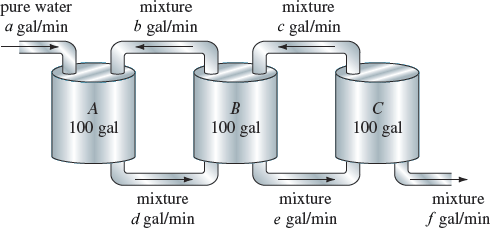
\includegraphics[width=0.5\textwidth]{figs/three-tanks}\quad 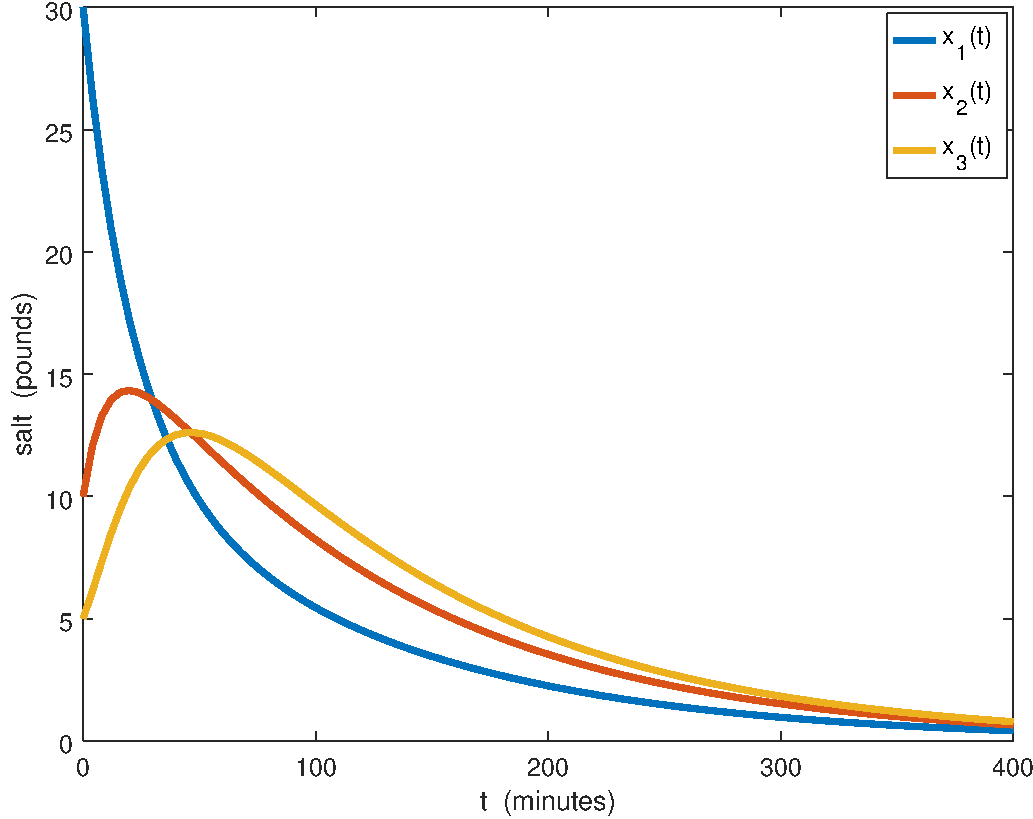
\includegraphics[width=0.5\textwidth]{figs/brines-xvt}}
\end{frame}


\begin{frame}{what does it look like?, cont.}

\begin{itemize}
\item variables $t,x_1,x_2,x_3$ \dots 4D? \dots unvisualizable!
\item alternate view is to suppress $t$

and plot in 3D $=x_1,x_2,x_3$
\item see code \href{https://bueler.github.io/math302/assets/codes/F23/brines.m}{\texttt{brines.m}}
    \begin{itemize}
    \item<2> uses \texttt{ode45}
    \item<2> \emph{rotatable} figure
    \end{itemize}
\end{itemize}

\vspace{-21mm}
\hfill 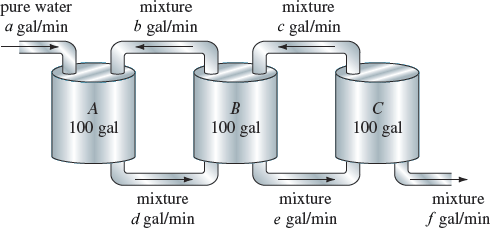
\includegraphics[width=0.42\textwidth]{figs/three-tanks}

\mbox{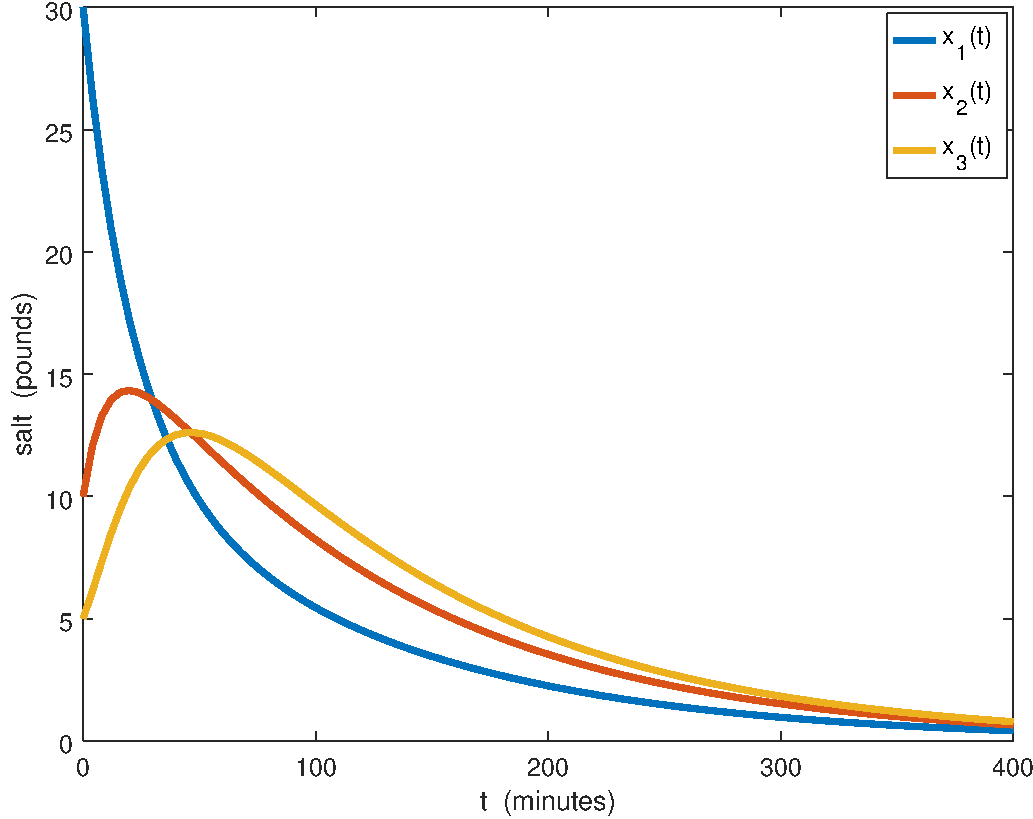
\includegraphics[width=0.5\textwidth]{figs/brines-xvt}\quad \includegraphics<1>[width=0.5\textwidth]{figs/brines-3d}\includegraphics<2>[width=0.5\textwidth]{figs/brines-3d-again}}
\end{frame}


\begin{frame}{these problems have solutions}

\begin{theorem}  Consider a linear system with initial values:
    $$\bX' = \bA \bX + \bF, \quad \bX(t_0)=\bX_0$$
Assume the entries in $\bA(t)$ and $\bF(t)$ are continuous.  Assume $\bX_0$ is a given vector.  Then there is one solution $\bX(t)$.
\end{theorem}

\bigskip
\begin{itemize}
\item so what?
\item it is a big deal!
\item \alert{you can make predictions}

from knowledge of current state \hfill $\bX(t_0)=\bX_0$

and laws about how things change \hfill $\bX' = \bA \bX + \bF$

to create one prediction \hfill $\bX(t)$
\end{itemize}
\end{frame}


\begin{frame}{these problems have \emph{general} solutions}

\begin{theorem}  Consider a \alert{homogeneous} linear system:
    $$\bX' = \bA \bX$$
There is a \alert{fundamental set} of solutions $\bX_1(t), \bX_2(t), \dots, \bX_n(t)$ so that any solution of the linear system is a linear combination:
    $$\bX(t) = c_1 \bX_1(t) + c_2 \bX_2(t) + \dots + c_n \bX_n(t)$$
\end{theorem}
\end{frame}


\begin{frame}{these problems have \emph{general} solutions 2}

\begin{theorem}  Consider a \alert{non}homogeneous linear system:
    $$\bX' = \bA \bX + \bF$$
Suppose $\bX_p(t)$ is one solution of this system.  Let $\bX_c(t)$ be the general solution to the associated homogeneous system $\bX' = \bA \bX$,
    $$\bX_c(t) = c_1 \bX_1(t) + c_2 \bX_2(t) + \dots + c_n \bX_n(t)$$
Then the general solution is
    $$\bX(t) = \bX_c(t) + \bX_p(t)$$
\end{theorem}
\end{frame}


\begin{frame}{like \#12 in \S8.1}

\begin{itemize}
\item \S8.2 shows how to solve homogeneous systems $\bX' = \bA \bX$
\item for now, you will be asked to \emph{check} solutions, as follows
\item \emph{example 10.}  verify that $\displaystyle \bX(t)=\begin{pmatrix} -1 \\ 1 \end{pmatrix} e^{-2t}$ is a solution of the linear system
    $$\bX' = \begin{pmatrix} 1 & 3 \\ 1 & -1 \end{pmatrix} \bX$$
\end{itemize}

\noindent \emph{solution.}

\vspace{35mm}
\end{frame}


\begin{frame}{like \#15 in \S8.1}

\begin{itemize}
\item \emph{example 11.}  verify that $\displaystyle \bX(t)=\begin{pmatrix} -1 \\ -6 \\ 13 \end{pmatrix}$ is a solution of the linear system
    $$\bX' = \begin{pmatrix} 1 & 2 & 1 \\ 6 & -1 & 0 \\ -1 & -2 & -1 \end{pmatrix} \bX$$
\end{itemize}

\noindent \emph{solution.}

\vspace{35mm}
\end{frame}


\begin{frame}{linear independent solutions}

\begin{itemize}
\item \emph{definition.} if $\bX_1(t),\bX_2(t),\dots,\bX_n(t)$ are  linearly-independent then we say they form a \emph{fundamental set}
\item you can check linear independence by checking that the \emph{Wronskian} is nonzero:
    $$W\left(\bX_1,\bX_2,\dots,\bX_n\right) = \det \begin{pmatrix} x_{11} & x_{12} & \dots & x_{1n} \\ x_{21} & x_{22} &  & x_{2n} \\ \vdots & & \ddots & \vdots \\ x_{n1} & x_{n2} & \dots & x_{nn} \end{pmatrix} \ne 0$$
\item above uses notation for entries:
    $$\bX_1 = \begin{pmatrix} x_{11} \\ x_{21} \\ \vdots \\ x_{n1} \end{pmatrix}, \bX_2 = \begin{pmatrix} x_{12} \\ x_{22} \\ \vdots \\ x_{n2} \end{pmatrix}, \dots, \bX_n = \begin{pmatrix} x_{1n} \\ x_{2n} \\ \vdots \\ x_{nn} \end{pmatrix}$$
\end{itemize}
\end{frame}


\begin{frame}{like \#17 in \S8.1}

\begin{itemize}
\item \emph{example 12.}  determine whether the vectors (solutions) form a fundamental set:
    $$\bX_1 = \begin{pmatrix} 1 \\ 1 \end{pmatrix} e^{-2t}, \quad \bX_2 = \begin{pmatrix} 1 \\ -1 \end{pmatrix} e^{-6t}$$
\end{itemize}

\noindent \emph{solution.}

\vspace{40mm}
\end{frame}


\begin{frame}{expectations}

to learn this material, just listening to a lecture is \emph{not} enough
     \begin{itemize}
     \item \emph{read} section 8.1
     \item do Homework 8.1
     \item from now on (\S 8.2, 8.4) we will focus entirely on \emph{homogeneous} systems
     \end{itemize}
\end{frame}

\end{document}
